\graphicspath{ {Figures/Pileup/Multiplier/} }

\chapter{Systematic Uncertainty Evaluations}

\section{Sensitivity of \texorpdfstring{$\omega_{a}$}{} to gain corrections}

\section{Sensitivity of \texorpdfstring{$\omega_{a}$}{} to pileup}

The systematic error on R due to the pileup construction consists primarily of two parts, the error due to misconstruction of the amplitude and the phase of the pileup. The error due to the amplitude misconstruction was calculated by scanning over a pileup multiplier parameter, from 90\% of the calculated pileup amplitude to 110\%, as shown in Figure \ref{fig:PileupMultiplier}. The sensitivity of R to the amplitude was determined to be 509.1 ppb per unit amplitude. The uncertainty of the pileup amplitude construction was determined by fitting a parabola to the \chisq as a function of the pileup amplitude, and taking the width of that parabola as the uncertainty. This width is determined as the distance in X for the \chisq to rise by 1 from the minimum, also calculated as $\sqrt{2/(\chi^{2})''}$.

\begin{figure}[H]
\centering
    \begin{subfigure}[t]{0.45\textwidth}
	    \centering
		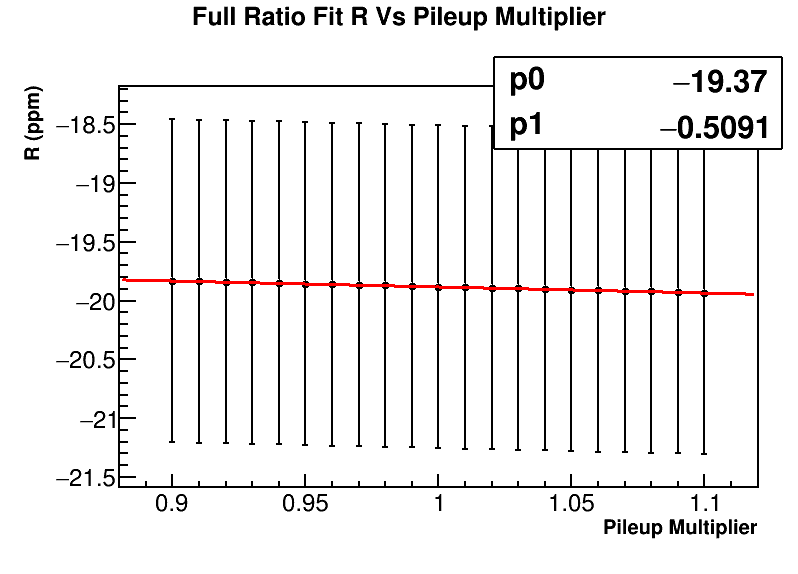
\includegraphics[width=\textwidth]{RatioCBO_R_Vs_PileupMultiplier_Canv}
	    \caption{Sensitivity of R vs the pileup amplitude. The slope is -509.1 ppb per unit amplitude.}
    \end{subfigure}
    \hspace{4mm}
    \begin{subfigure}[t]{0.45\textwidth}
	    \centering
		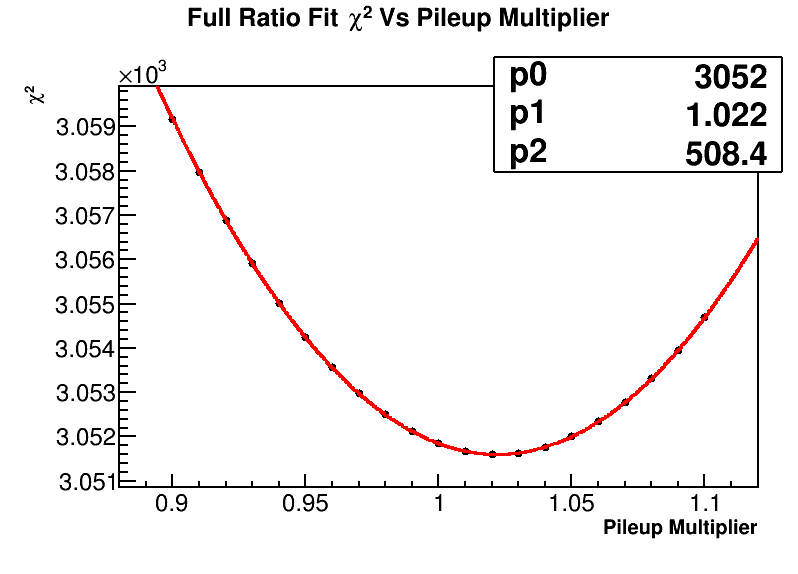
\includegraphics[width=\textwidth]{RatioCBO_Chi2_Vs_PileupMultiplier_Canv}
	    \caption{Plotted is the fitted \chisq vs the pileup amplitude. The fit equation used was $p2 \times (x - p1)^{2} + p0.$ The minimum therefore lies at 1.022.}
    \end{subfigure}
\caption[PileupMultiplier]{The significant plots to determine the pileup amplitude systematic error.}
\label{fig:PileupMultiplier}
\end{figure}

This corresponds to an uncertainty of $\sqrt{1/508.4} = 0.0444$ or 4.44\%. The minimum of the \chisq plot of 1.022 lies at approximately .5$\sigma$ away from 1, which is consistent and nice to see. Then, calculating the systematic error on R due to the pileup amplitude construction as 
	\begin{align}
		\delta R_{pm} = \delta\alpha_{pm} \times \frac{dR}{d\alpha_{pm}}
	\end{align}
where $\delta\alpha_{pm}$ is the uncertainty on the pileup amplitude, the systematic error on R is calculated as 509.1 pbb $\times 0.0444 = 22.6$ ppb.






The shape of the energy spectrum of the pileup was not taken to be the unceratiny because the shape is off blah blha

This uncertainty takes care of the triples because..



The pileup phase sysetematic error is calcualted as...





A third part is the error due to unseen pileup which...





\section{Sensitivity of \texorpdfstring{$\omega_{a}$}{} to lost muon function shape}

\section{Sensitivity of \texorpdfstring{$\omega_{a}$}{} to CBO function}

\section{Sensitivity of \texorpdfstring{$\omega_{a}$}{} to VW function}

\section{Sensitivity of \texorpdfstring{$\omega_{a}$}{} to various effects}

\section{Final Systematic Uncertainty Table}

\section{Final Results}
